\chapter{Preliminary Results}
\label{chap:prelim}

\begin{figure}
	\scalebox{0.75}{
	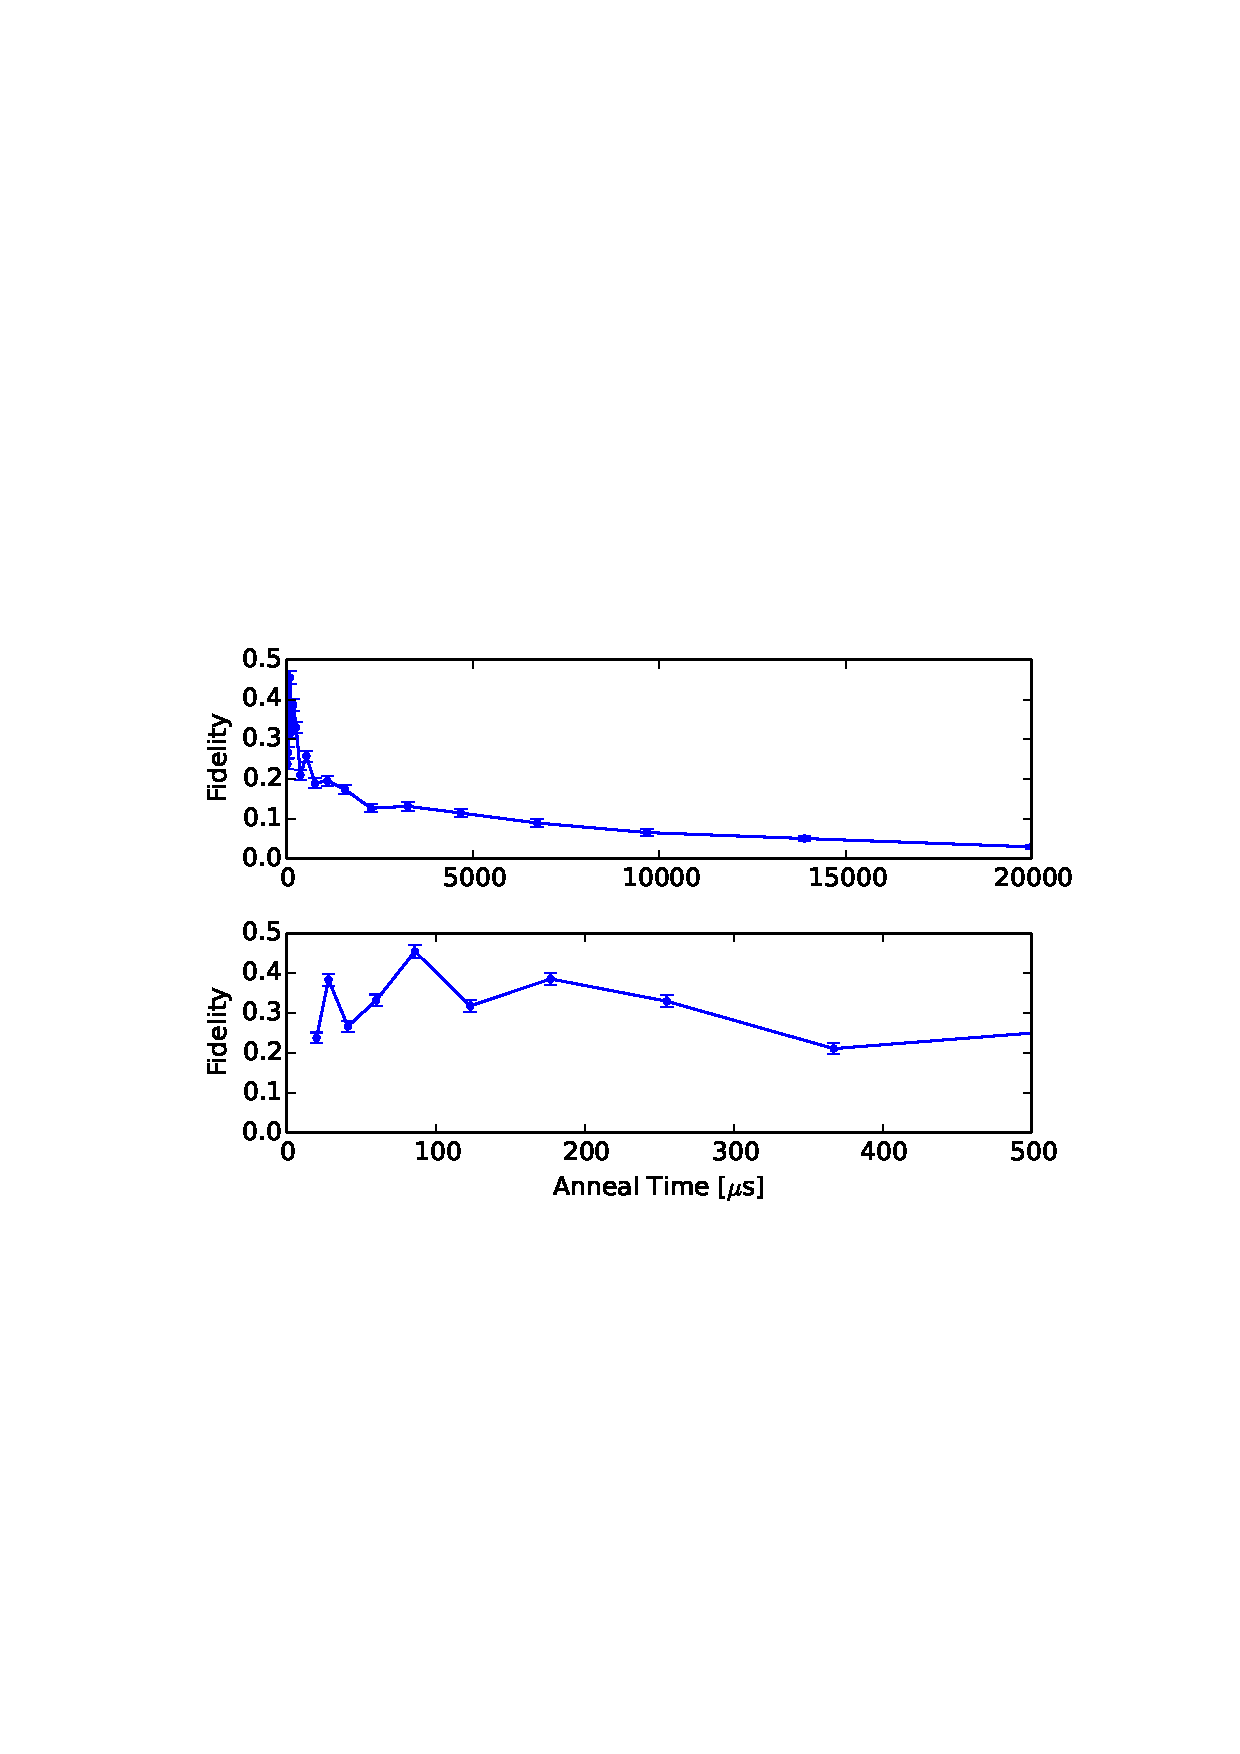
\includegraphics[bb=0 0 800 600]{img/6_018_2_fidelity.png}
}
	\caption[Fidelity vs Time]{Plot of the fidelity as a function of annealing time for the Hamiltonian ``6\_018'' both linear and log-scaled x-axis.}
	\label{fig:fidelity}
\end{figure}

Preliminary results were gathered on a sample quasi-random Hamiltonian called ``6\_018''.  This problem Hamiltonian was built up of clusters of clause sub-Hamiltonians in the same way as a SAT solver Hamiltonian would be, although ``6\_018'' does not encode a actual SAT problem.  This Hamiltonian was simple to generate and allowed us to verify our procedure for analyzing AQC results.
Data was collected in a series of evolutions at annealing times ranging from 20 $\mu$s to 20 ms.  Each evolution consists of choosing an anneal time and programming the problem Hamiltonian onto the hardware, then annealing 1000 times successively and reading out the final states.  We call each of these individual evaluations a \emph{read}, and a whole sequence of reads with the same programmed Hamiltonian a \emph{run}.  Any programming error (see \ref{sec:noise}) in the Hamiltonian should be the same between reads and differ between runs.
The estimated fidelity at each anneal time is the fraction of reads that returned (one of the) ground state(s).  The error is estimated by modelling the read process as a biased coin, with a probability $p$ of returning heads (the ground state), and a probability $1-p$ of returning tails (any other state).  This gives us a binomial distribution, which has a variance of $np(1-p)$ for $n$ trials.  

\begin{itemize}
	\item For short annealing times, why does the fidelity appear insensitive to annealing time?
	\item For long annealing times, why does the fidelity decrease with increasing annealing times?
	\item Is the short time fidelity dominated by the Hamiltonian programming noise?
	\item Is there significant drift in the fidelities after programming (i.e. read noise)?
	\item Does the Hamiltonian fidelity depend strongly on the number of coupling values?
\end{itemize}

or in short: Our theoretical model of quantum annealing suggests that the fidelity at T = 0 should be $2^{-N}$ for an $N$ spin Hamiltonian and increase as the annealing time increases, reaching approximately $1$ in the limit of $T \rightarrow \infty$ (as shown in Figure \ref{fig:simulated_anneal}).  Instead, the fidelity at our smallest accessible annealing time is already ``large'' and is seemingly insensitive to annealing time until the fidelity begins to \emph{drop} (as shown in Figure \ref{fig:fidelity}).

\emph{Why does the machine behave in this way contrary to our expectations?  Why does the short-anneal fidelity vary so much, and why does the long-anneal fidelity decrease rather than increase?}

\section{Short-time Evolution}


\section{Long-time Evolution}
For a purely quantum system the fidelity should increase in the limit of increasing annealing time.  What we see instead in the actual data is that the fidelity appears to approach zero as the annealing time increases.  The physical computer is not an ideal quantum system, so to model it correctly we need to account for noise and decoherence sources.

We should fit this decreasing fidelity, or perhaps the population histogram, to some sort of model of thermal noise.  Then we could determine the energy leakage, maybe.


\begin{figure}
	\scalebox{0.35}{
		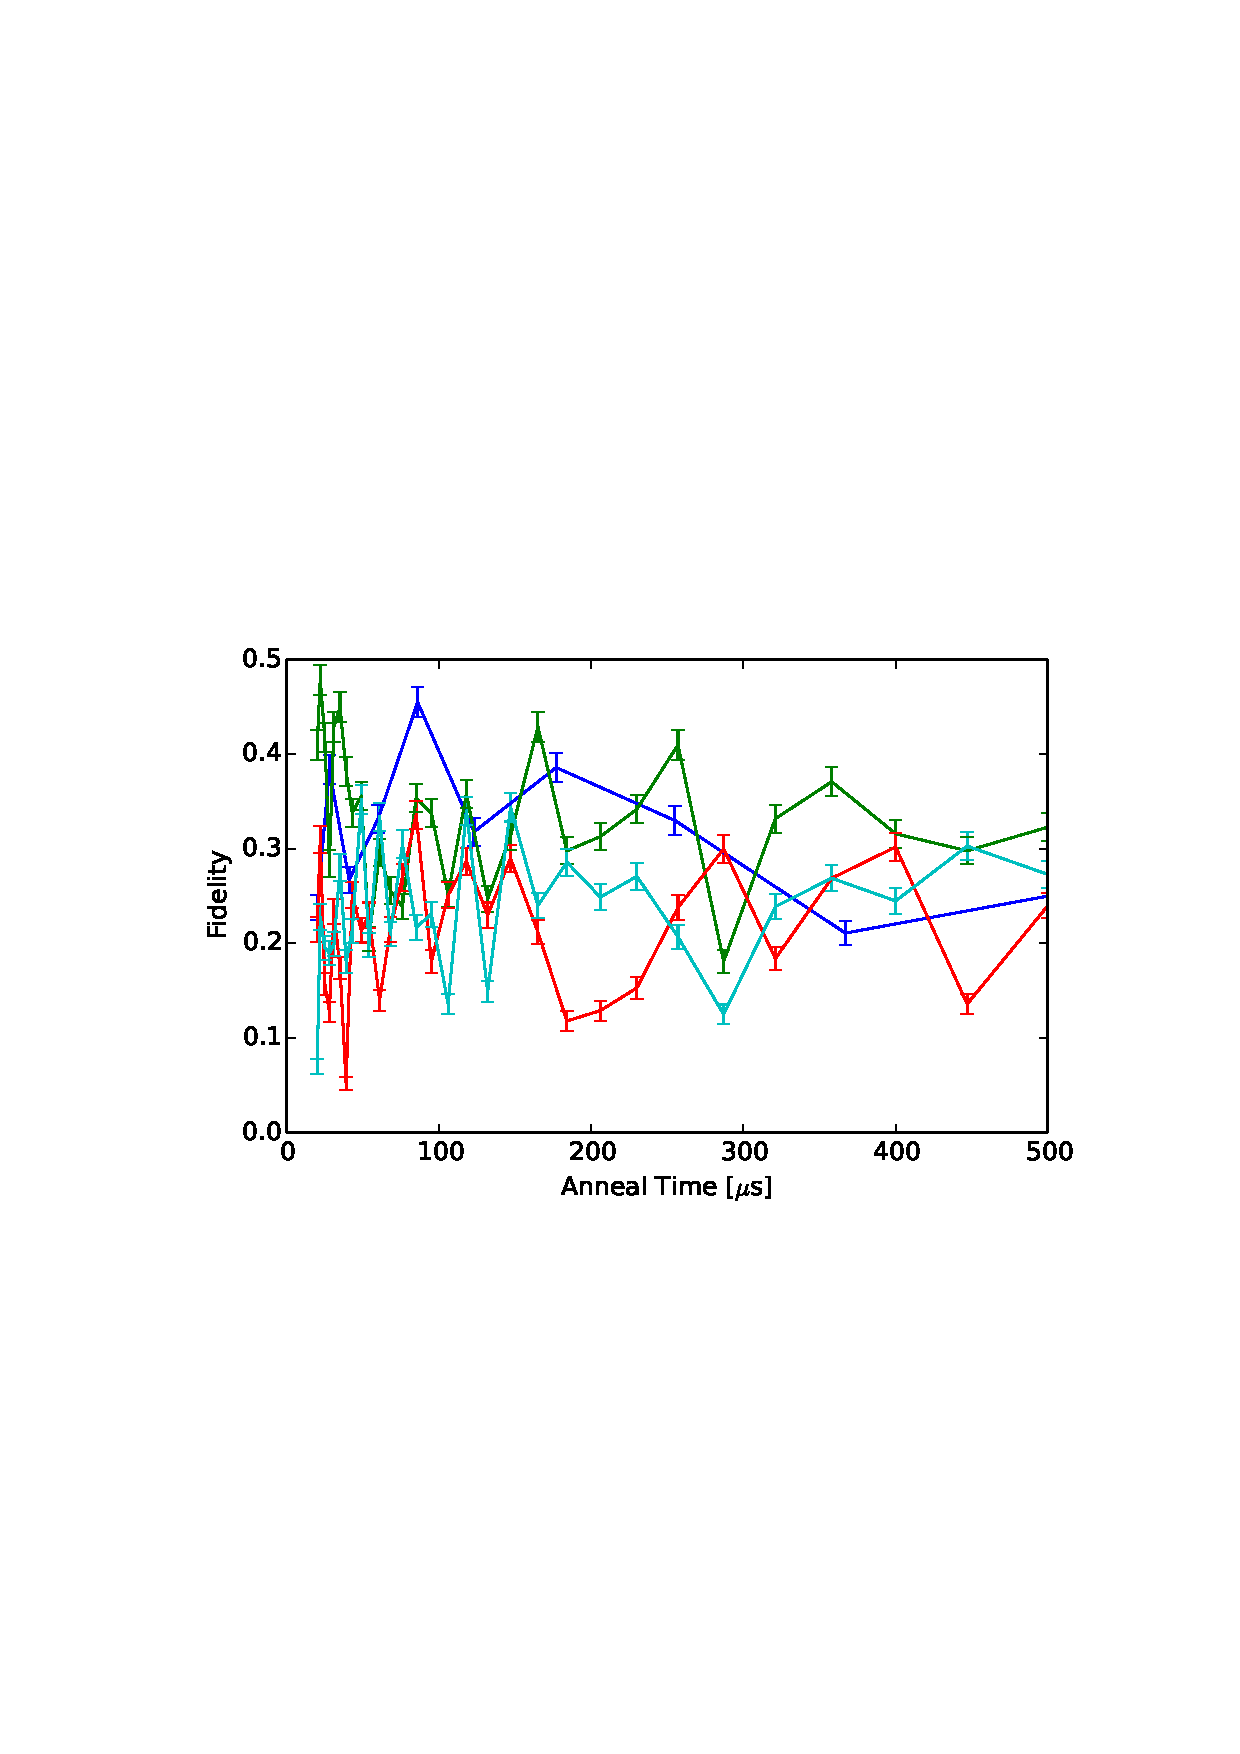
\includegraphics[bb= 0 0 745 382]{img/6_018_comparison.png}
	}
	\caption[Short Time Fidelities]{The fidelity as a function of time for the Hamiltonian ``6\_018'' for several different machine runs.  Each data point consist of 1000 machine reads.  Notice the spread between machine runs is outside of the error bars.}
	\label{fig:short_fidelity}
\end{figure}

\begin{figure}
	\scalebox{0.75}{
		\includegraphics[bb= 0 0 800 600]{img/4_5_hist.png}
	}
	\caption[Short Time Fidelity Histogram]{Histogram of the fidelities found for all annealing times  $< 500 \mu$s.  Notice the gaussian like structure.}
	\label{fig:fid_hist}
\end{figure}

\begin{figure}
	%\scalebox{0.75}{
	%	\includegraphics[]{}
	%}
	\caption[Simulation of Schr\"odinger's Equation]{Numerical integration of Schr\"odinger's Equation for the Hamiltonian ``k44'' showing the fidelity increasing to a plateau as the annealing time increases.}
	\label{fig:simulated_anneal}
\end{figure}

\begin{figure}
	%\scalebox{0.75}{
	%	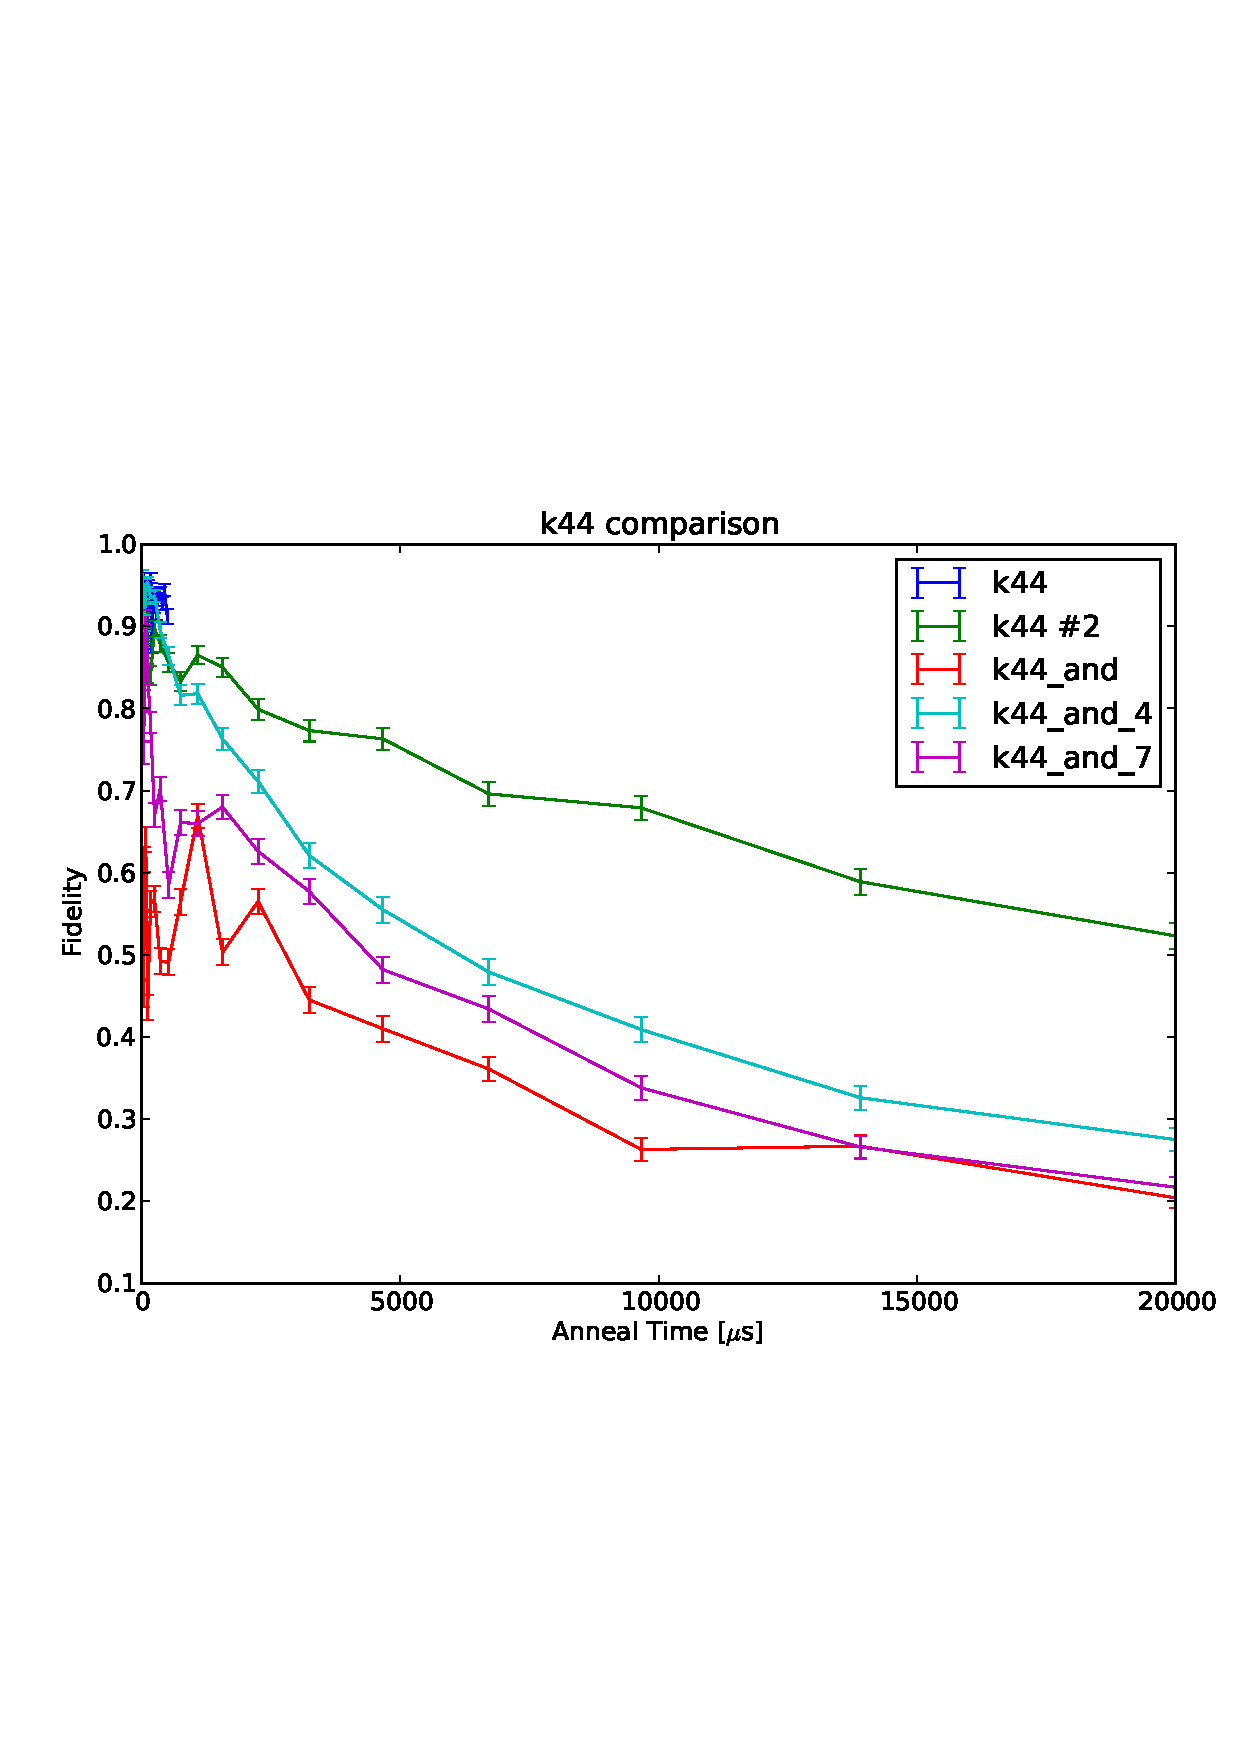
\includegraphics{img/k44_comparison.pdf}
	%}
	\caption[Long Time Anneal]{Machine data from Hamiltonian ``k44'' with 100 runs of 1000 reads showing the Hamiltonian noise at short times and the fidelity drop at long anneal times.}
	\label{fig:k44_long}
\end{figure}
